\section{Introduction}
This open source project is development of wireless data collecting equipment. The project is in cooperation with the geologist Dr .Andrew D. Wickert (seen in figure \ref{fig:andrewWickert}), who has need for affordable and light-weighted field instrumentation for his research. That's why he developed Arduino-based low-power field environmental data logger, as seen in figure \ref{fig:BottleLog}. He sought assistance to Reykjavik University for help with development of communication module that fits his data logger.\\
So the main goal with this project is design of Arduino based communication module that sends data through GSM network to HTTP server. With this accomplished and later on merge with Andy's data logger there will be affordable light-weighted equipment that is not available commercially. The solution will also be highly modifiable because it's open source project.

\begin{figure}
\centering
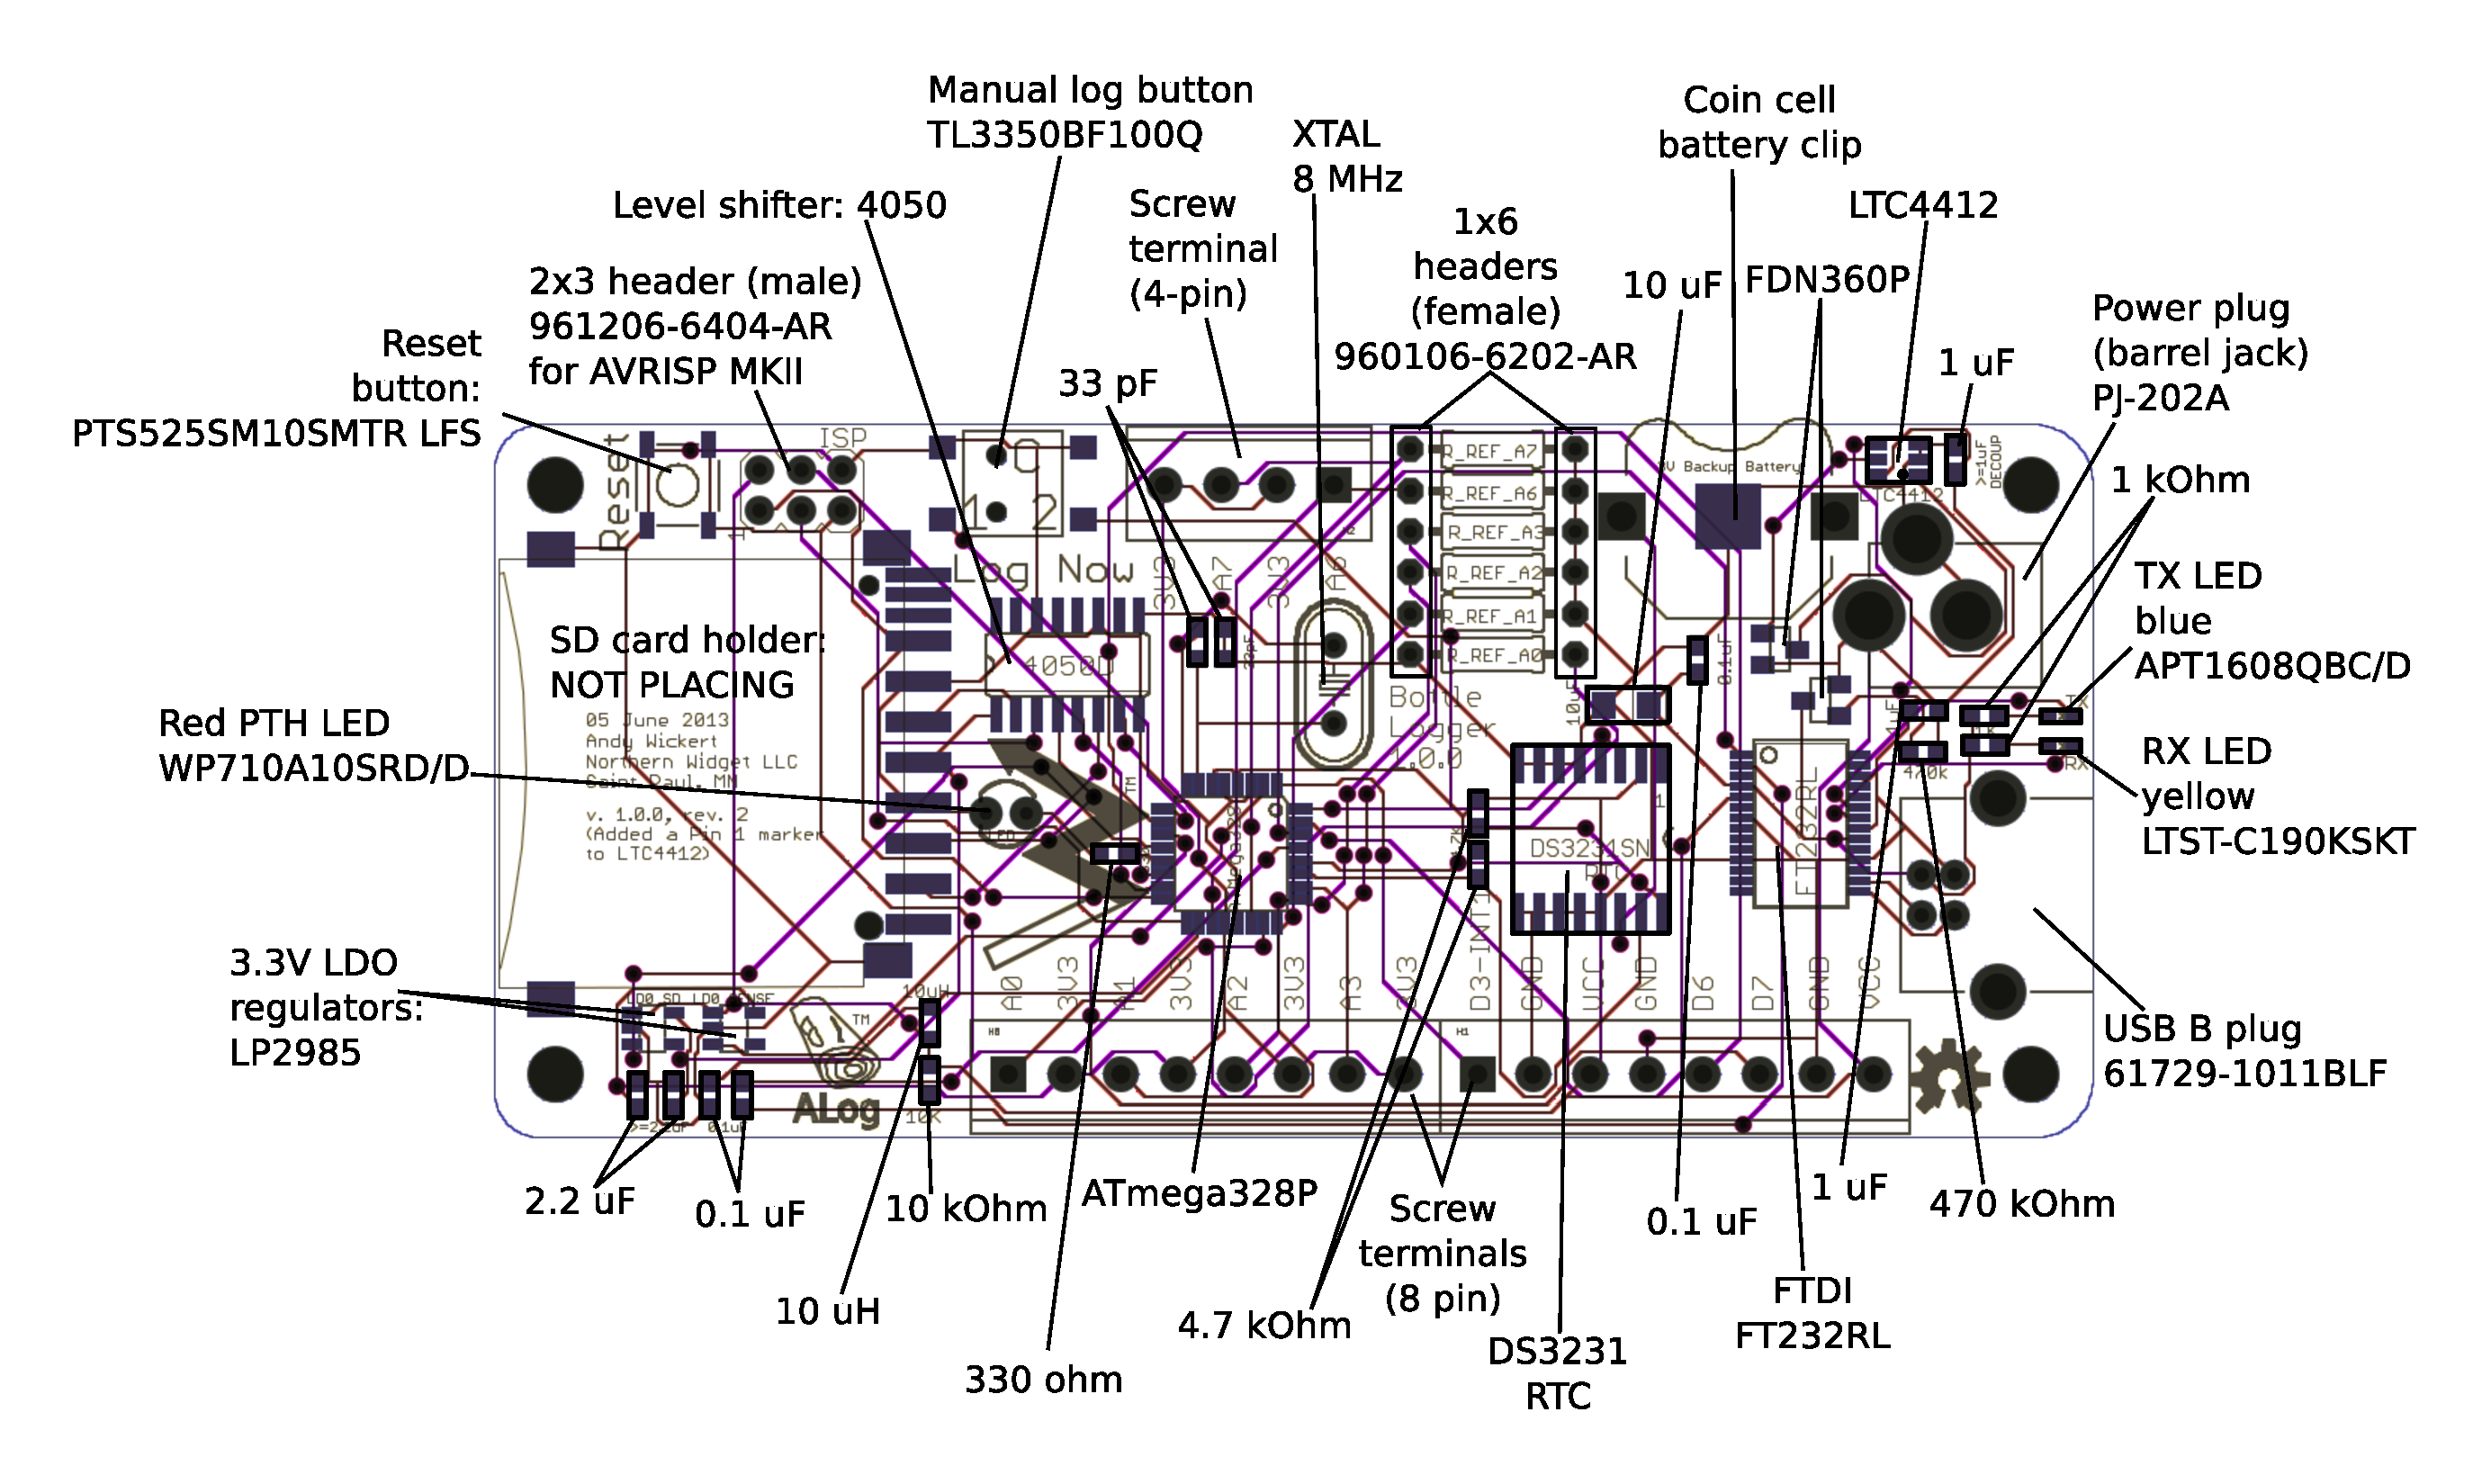
\includegraphics[height=5.7cm]{graphics/ALog_drawing.PDF}
\caption{Arduino-based low-power field environmental data logging platform: hardware schematics and circuit board layouts\label{fig:BottleLog}\cite{ALog-BottleLogger}}
\end{figure}

\subsection{Background}
Data sampling is well know method to help scientist to understand nature's behavior. Back in days, scientist had to sample data in real time on the field by writing measurements down to log book. Later on with automatic measurement equipment they where able to leave it behind in the field, then come back later and collect the data from them to process. Later on with impact of wireless communication technology the automatic measurement equipment the scientist were able to access data in real time to process.\\
Similar equipment that is available to day that fulfills the requirements of being light-weight, inexpensive and has long-range transmit capabilities is not available. The equipment that is capable of long range communications through GSM network can be seen in figures \ref{fig:a} and \ref{fig:b} and they cost about \$3000. Then there is cheaper equipment that costs around \$500 as in figures\ref{fig:c} and  \ref{fig:d} but the downfall with them is that they have limited wireless range up to 300 m.

\begin{figure}[H]
  \centering
  \subfloat[\$3500 \label{fig:a}\cite{WeatherShop2014}]
  {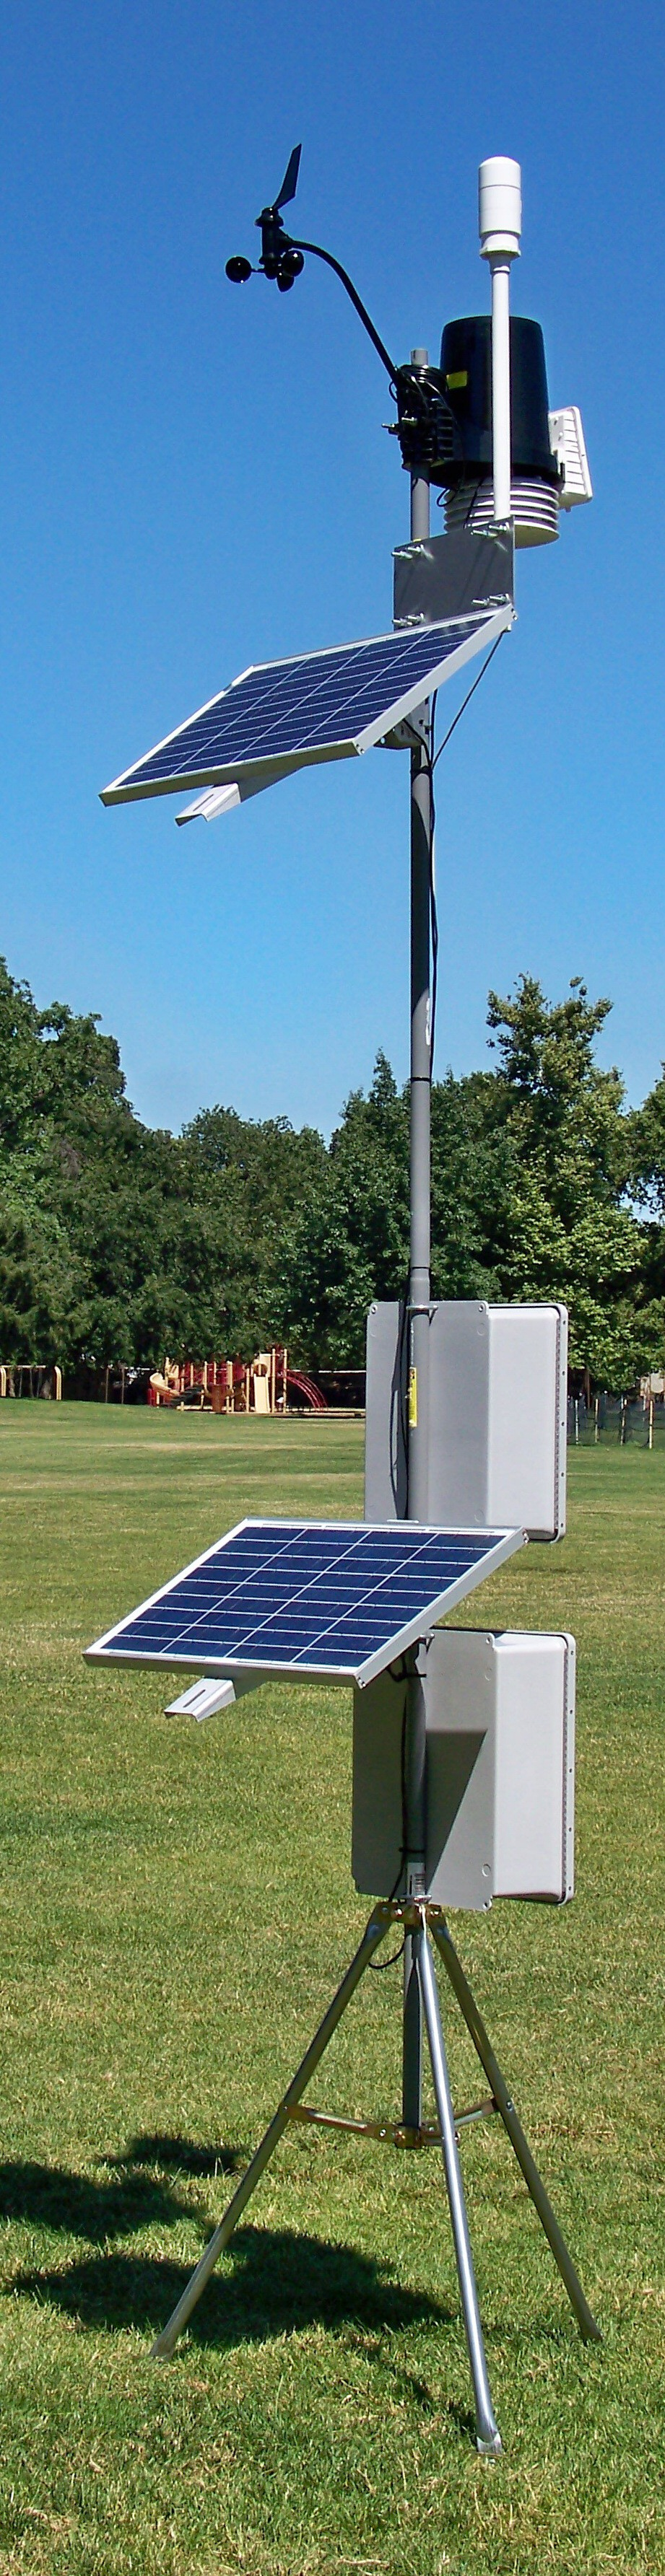
\includegraphics[height=6.5cm]{graphics/cellular_weather_station}}\quad
  \subfloat[\$2800 \label{fig:b}\cite{TexasWeatherInstruments2014}]
  {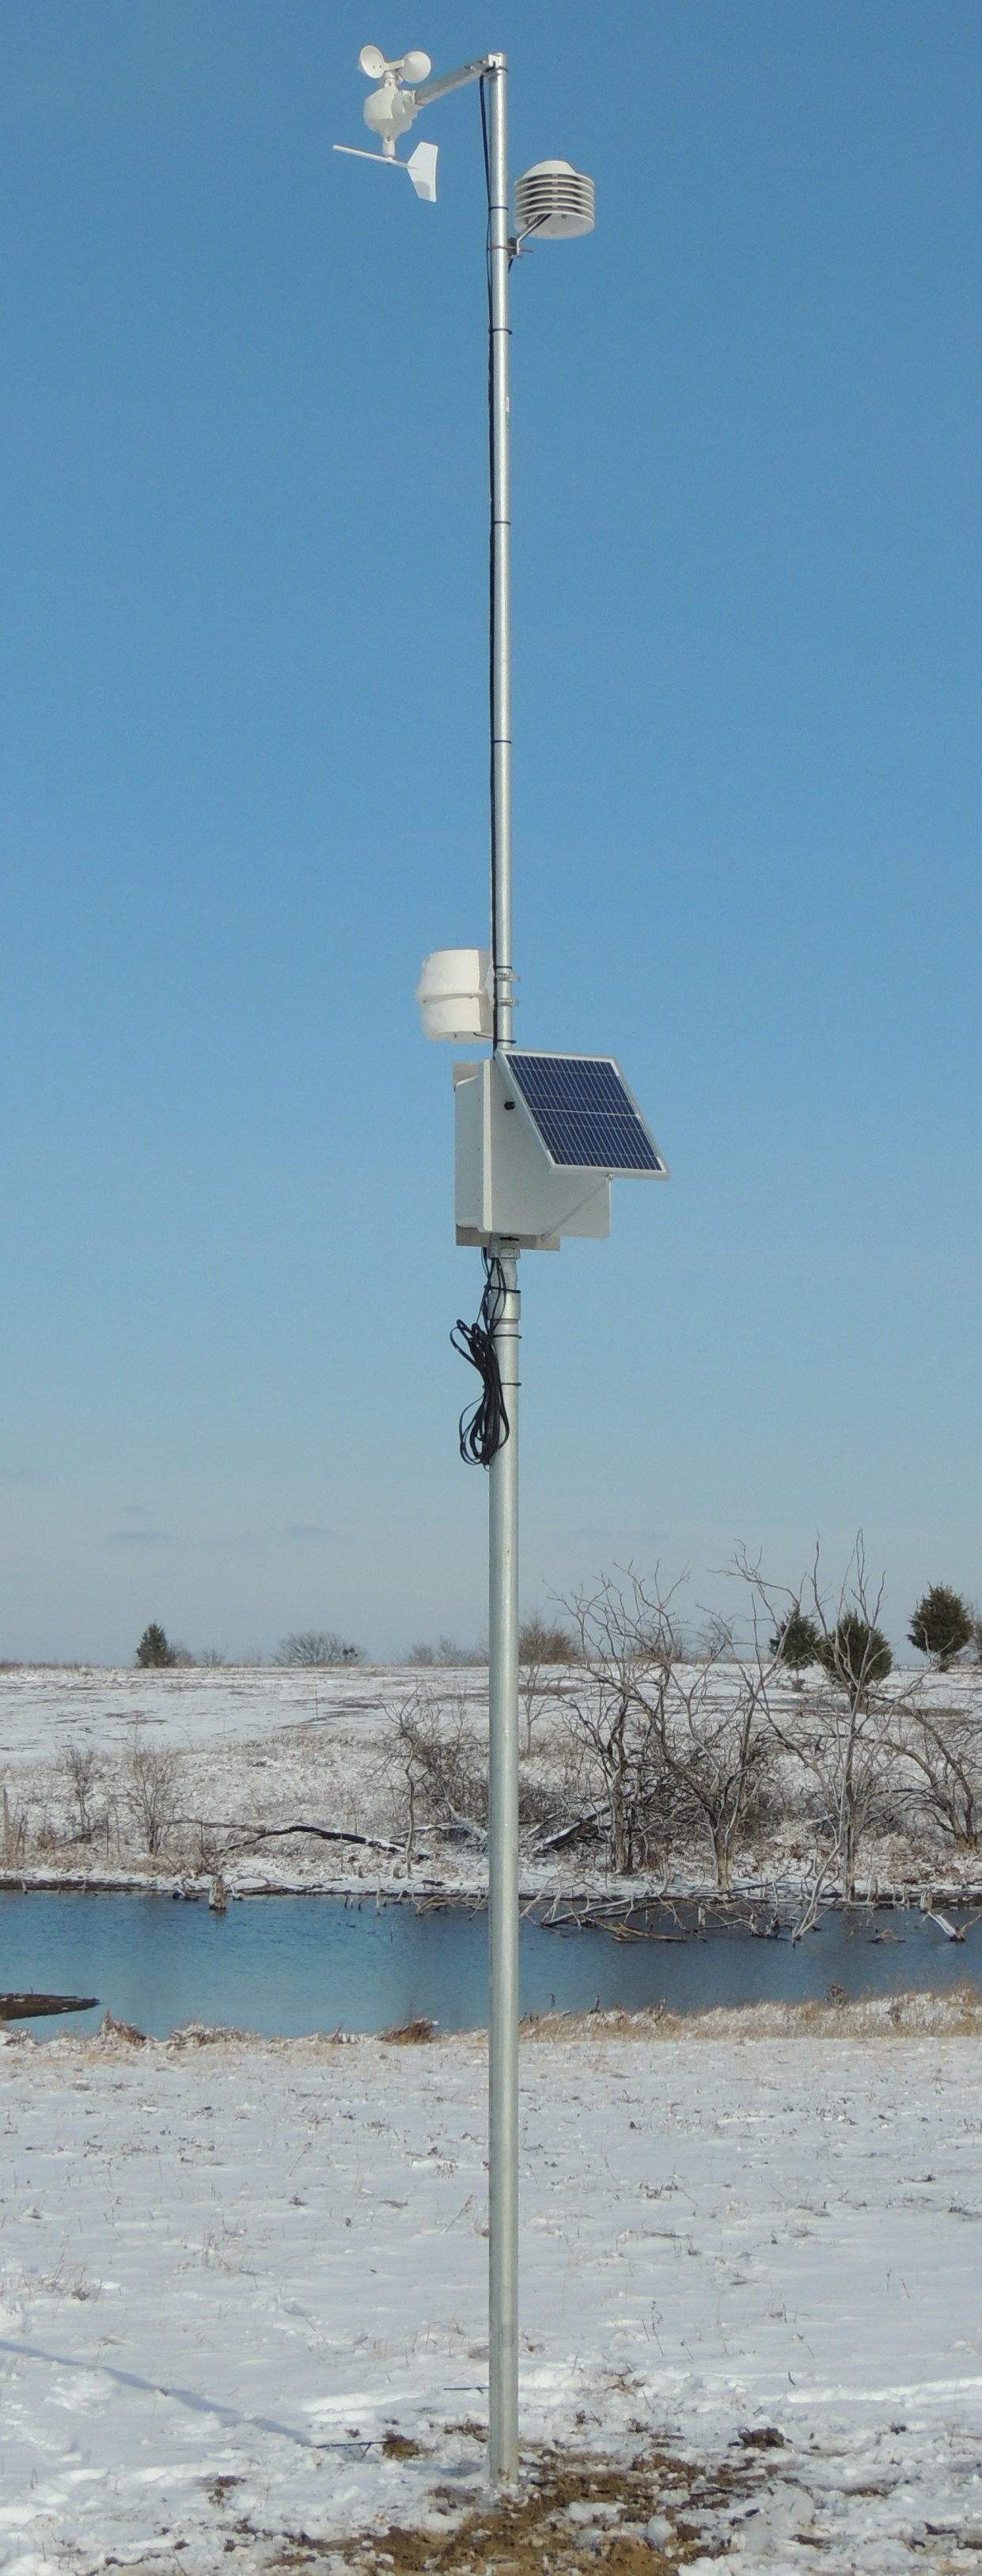
\includegraphics[height=6.5cm]{graphics/RWS-Snow}}\quad
  \subfloat[\$658 \label{fig:c}\cite{Scientific2014}]
  {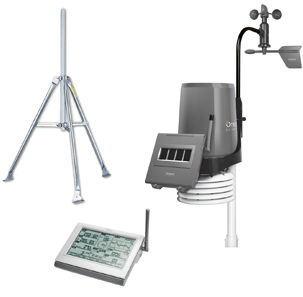
\includegraphics[height=4cm]{graphics/Oregon_Scientific_Pro_weather_system}}\quad
  \subfloat[\$595 \label{fig:d}\cite{Davis2014}]
  {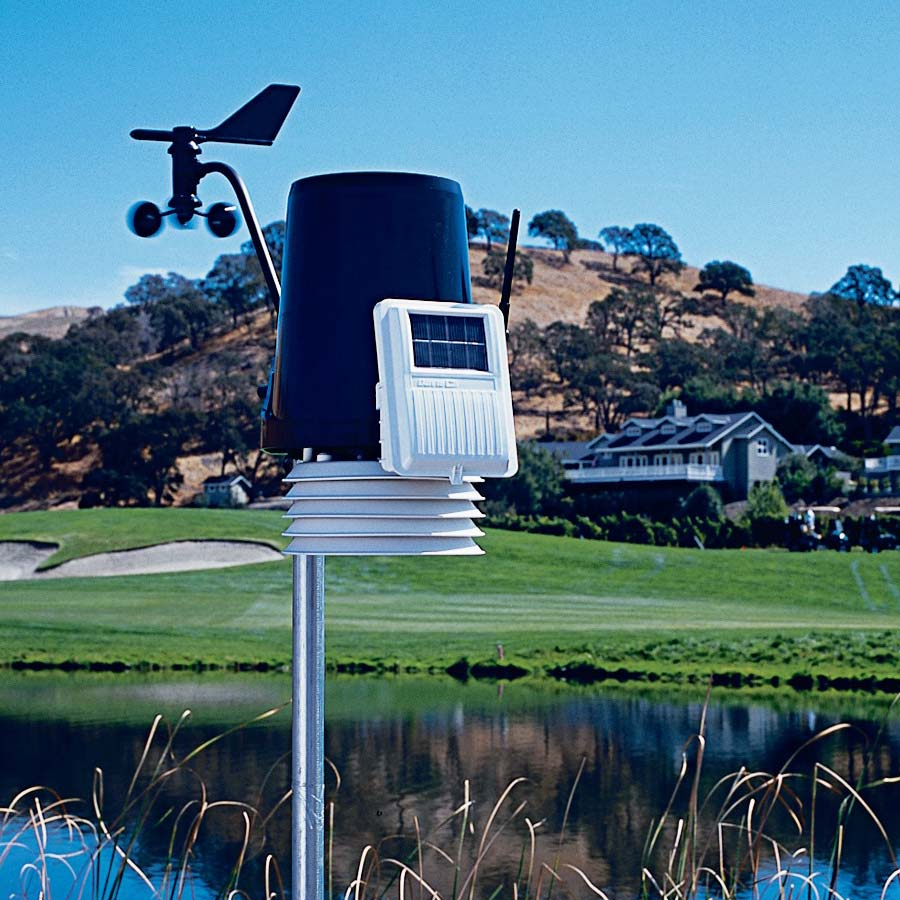
\includegraphics[height=4cm]{graphics/Davis_Vantage_Pro_2}}  
  \caption{Various price of portable weather stations}
  \label{fig:1}
\end{figure}

With that in mind the concept with this project is to make long-range communication data logger that is affordable. That can have good impact on the scientific communities were budgets are often limited. It can also result in more dens coverage in data logging. 

\subsection{Requirements}
\begin{table}[h!]
	\caption{FR-DP}
	\label{tbl:FRDP}
\begin{tabular}{|p{8cm}|p{8cm}|}
		\hline \textbf{Functional requirements (FR):} & \textbf{Design parameter (DP):} \\ 
		\hline 1) Collect measurable data &   Get temperature with TMP36 sensor\\
		\hline 2) Store data local &   Write temperature values to Arduino MEGA EEPROM \\
		\hline 3) Keeps data for x time &  Arduino MEGA \cite{arduinoMega} has 4kB of EEPROM \\
		\hline 4) Runs on own power source & Have battery pack and minimize power consumption \\ 
		\hline 5) IP67 proof &   Fit all hardware into IP67 fiber box\\
		\hline 6) Sent data wireless through GSM network & Send Jason formated data trough GSM shield \\ 
		\hline 7) Store data on server & Setup HTTP API server \\ 
		\hline 8) Modular Design & Well planed software design architecture \\ 
		\hline
	\end{tabular}
\end{table}

The most challenging requirements from table \ref{tbl:FRDP} is the software design. It's very critical to make the hole project modular. Solution to that is decrepit in DP7. Additionally there were added 3x wireless-sensor module to expand the coverage of the mother-base. They use Pololu Wixel to communicate to mother hub. Then the mother hub samples data from them and sends through GSM network to a HTTP server.

